Так как в нашем случае лабораторный источник рентгеновского излучение имеет
некое угловое  (см. \ref{sec:source_section}) и спектральное распределение
для исследования материалов требуется наличие монохроматора, принцип действия которого
был описан в разделе \ref{sec:single_crystal_section}. Такой луч, отражаясь от
кристалла (схема на рис. \ref{ris:single_crystal_schem_lamtet}), разделятся в пространстве
в соответствие с условием Брэгга (разные длины волн отражаются под разными углами).
% В рамках последовательно движения от более простого к более сложному мы не оставили без внимание
% получения угловой зависимости интенсивности (рис. \ref{ris:single_crystal_schem_exp}), чтобы соотнести
% выражение для описания спектра трубки (\ref{eq:source_spectral}) с экспериментальным.

\begin{figure}[H]
  \centering
  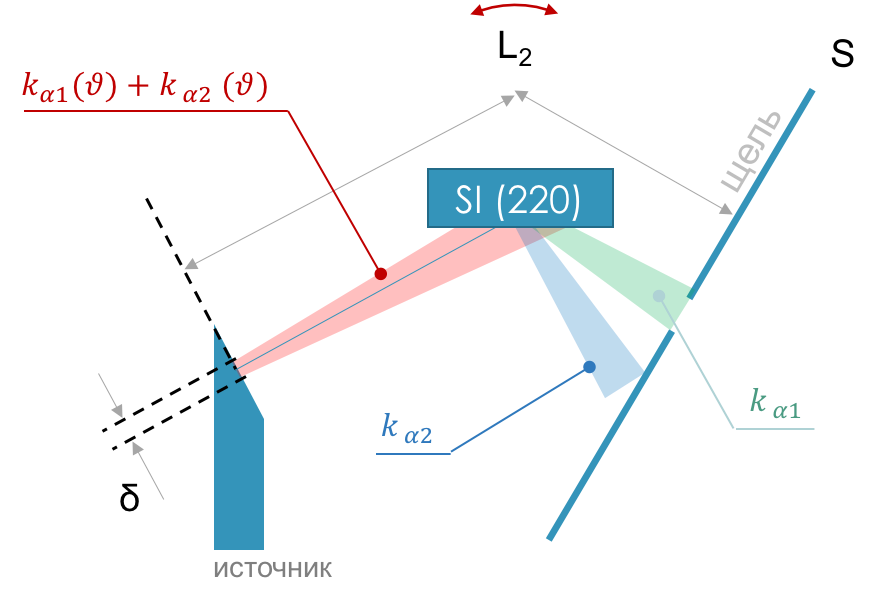
\includegraphics[width=0.5\textwidth]{images/single_crystal_schem_exp.png}
  \caption{Схема однокристального эксперимента, лучи с разной энергией отражаются под разными углами
  в соответсвии с условием Брэгга}
  \label{ris:single_crystal_schem_exp}
\end{figure}

Интенсивности отражения рентгеновского излучения приведенная на рис. \ref{ris:zero_exp} может быть
получена в зависимость от угла поворота кристалла или движение детектор с щелевым устройством,
задающим его апертуру. В качестве кристалла был взят монокристалл кремния Si(220).

\begin{figure}[H]
  \centering
  \subfloat[]{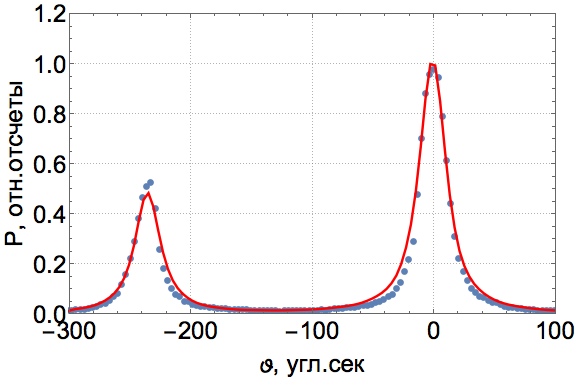
\includegraphics[width=0.45\textwidth]{images/single_cr_exp_s_005mm.png}}
  \hfill
  \subfloat[]{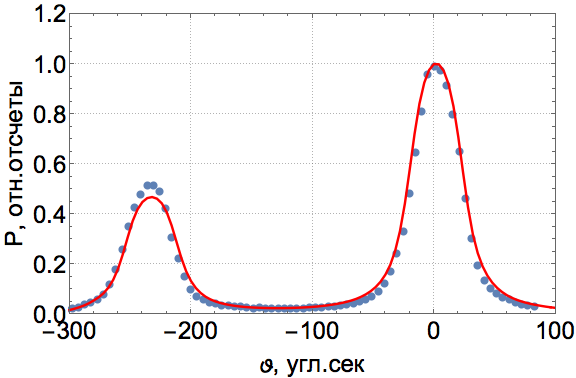
\includegraphics[width=0.45\textwidth]{images/single_cr_exp_s_02mm.png}}
  \caption{Угловая зависимость интенсивности после отражения характерестического излучения от кристалла монохроматора.
   (красная линия) - расчет, (синие точки) - эксперимент для (a) $S = 50$ мкм; полуширина $k_{\alpha 1}$ линии ($\vartheta=0$)
   составляет около 30 угл.сек., (b) $S = 200$ мкм; полуширина $k_{\alpha 1}$ линии ($\vartheta=0$)
   составляет около 50 угл.сек.}
  \label{ris:zero_exp}
\end{figure}

Результат сравнения экспериментальной картины дифракции и моделирования
подтверждает правильность выбора функции спектра рентгеновской трубки (\ref{eq:source_spectral}),
которая представляет из себя сумму двух функций Лоренца, взятых с весовыми коэффициентами.
Так же можно пренебречь наличием тормозного излучения спектра трубки.
